\documentclass[11pt]{article}

\usepackage{graphicx}
\usepackage{framed}
\usepackage{hyperref}

\marginparwidth 0.5in 
\oddsidemargin 0.25in 
\evensidemargin 0.25in 
\marginparsep 0.25in
\topmargin 0.25in 
\textwidth 6in \textheight 8 in

\begin{document}
\hfill\vbox{\hbox{Jude Shin, Torrey Zachs}
		\hbox{CSC 321, Section 07}	
		\hbox{Module 2: Block Ciphers}	
		\hbox{\today}}\par

\bigskip
\centerline{\Large\bf Lab 02: Symmetric Key Cryptography Exploration}\par
\bigskip

This lab explores symmetric key cryptography security with both Electronic Codebook (ECB) and Cipher Block Chaining (CBC) modes. This lab also demonstrates the limits and exploitations of each, as well as a performance study of public versus symmetric key algorithms. This lab was completed using {\tt Python} and {\tt PyCryptodome}. All the code can be found in the \href{https://github.com/jude-shin/CSC\_321}{remote github repository}

% ============================================================================
\section*{Environment}

If you want to run and test the code, a virtual environment should first be set up with the correct requirements. This ensures that there is consistency between all of the packages used within this project.

\begin{itemize}
	\item Make a virtual environment (venv) with python.

		\verb|$ python3 -m venv .venv|

	\item Activate the venv.

		\verb|$ source .venv/bin/activate|

	\item Install the requirements using pip.

		\verb|$ pip install -r requirements.txt|

	\item Whenever you are done you can deactivate the venv.

		\verb|$ deactivate|

\end{itemize}

% ============================================================================
\section*{Task 1: Modes of Operation}
\subsection*{Abstract}
The main datatype used was the \verb|bytes| datatype, which could be treated as a fixed array of bytes; this datatype could be iterated over, and indexed, making it easy to locate particular parts of an encrypted or decrypted message. The path to the bmp that the user wants to encrypt is listed as the first command line argument. Both methods of single key encryption use "blocks" of data. In our case, we chose to use 128 but (8 byte) chunk sizes. In our example, we will encrypt some bmp images. In both cases, the first 54 bytes were removed as they were the bmp headers. Then the rest of the data was padded to be divisible by the chosen block size.

\subsection*{Code Breakdown}
\subsubsection*{task1.py}

The python script \verb|task1.py| executes two functions, one to encrypt a file with ECB, and one to encrypt a file with CBC. 

\begin{framed}
\begin{verbatim}
if __name__ == '__main__':
    if len(sys.argv) == 2:
        plaintext_file: str = sys.argv[1]

        encrypt_bmp_with_ecb(plaintext_file)
        encrypt_bmp_with_cbc(plaintext_file)

    else:
        print('One cmd line arg required!')
\end{verbatim}
\end{framed}

\subsubsection*{ECB Code}

ECB takes in the

\subsubsection*{CBC Code}

lorum ipsum crap or whatever

\subsubsection*{PKCS\#7 Code} 

The PKCS padding scheme adds a number of bytes to the end of the data, ensuring that the encryption algorithm has even blocks to work with. Let the number of remaining bytes that were filled be \verb|(k)|. Each byte that is appended to the end of the data is the integer \verb|k| represented as a byte. This, of course, is a well defined padding system up to padding of 255 extra bytes.

\begin{framed}
\begin{verbatim}
# pad text bytes with pkcs#7 padding
def add_padding(text: bytes, block_size: int) -> bytes:
    # Get the remainder that is needed to become a multiple of block_size
    k: int = block_size - len(text)%block_size

    # k(byte) will be repeated k times
    single_byte: bytes = k.to_bytes(1, 'big')
    padding: bytes = single_byte * k

    # Append the padding to the end of the text 
    return text + padding 

# remove a padded text bytes with pkcs#7 padding
def strip_padding(text: bytes) -> bytes:
    # Read the last block (should be an int)
    k: int = text[-1]

    # If the number that are in the last k bytes does not match up
		# , then there was no padding (or a padding of 0)
    for i in range(k):
        if (k != text[-(i+1)]):
            return text 

    # Remove the last k bytes in text 
    return text[:-k]
\end{verbatim}
\end{framed}

\subsubsection*{Utilities Code}

Some helper functions were shared between the two encryption methods like reading and writing bytes to a file. Note that we open the file with the binary mode (indicated by the 'b') to indicate that we want a \verb|bytes| datatype instead of a file object.

\begin{framed}
\begin{verbatim}
def read_bytes(filename: str) -> bytes:
    with open(filename, 'rb') as f:
        return f.read()

def write_bytes(filename: str, text: bytes) -> None:
    with open(filename, 'wb+') as f:
        f.write(text)
\end{verbatim}
\end{framed}

\subsection*{Reproduction}

Running both encryption processes on a given bmp is as simple as activating the venv, and then running \verb|task1.py| with the file to be encrypted.

\verb|$ python task1.py ./path/to/image.bmp|

\subsection*{Results}
\subsubsection*{CBC Results}
\subsubsection*{Results Results}

% ============================================================================
\section*{Task 2: Limits of Confidentiality}
\subsection*{Abstract}

% ============================================================================
\section*{Task 3: Performance Comparison}
\begin{figure}
	\centering
	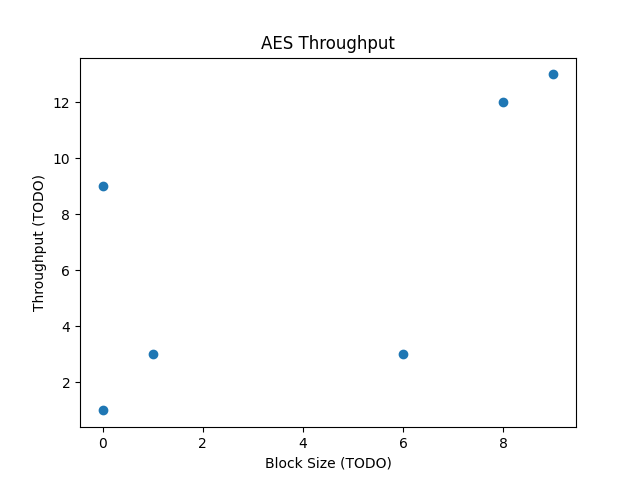
\includegraphics[width=0.8\textwidth]{./plts/aes.png}
	%\caption{}
	\label{fig.1: Performance of AES}
\end{figure}

\begin{figure}
	\centering
	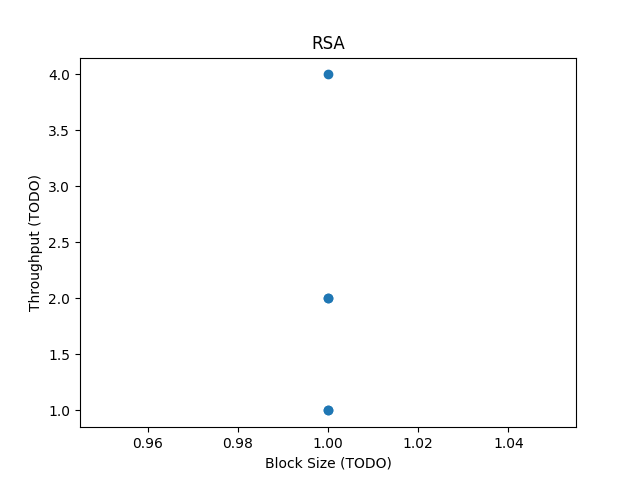
\includegraphics[width=0.8\textwidth]{./plts/rsa.png}
	%\caption{}
	\label{fig.2: Performance of RSA}
\end{figure}

% ============================================================================
\section*{Questions}
\subsection*{question 1}
\subsection*{question 2}
\subsection*{question 3}

\end{document}
